\appsection{Спецификация блока спутника типа CubeSat}{attachement_cubesat_design}

\begin{sidewaysfigure}[htbp]
	\centering
	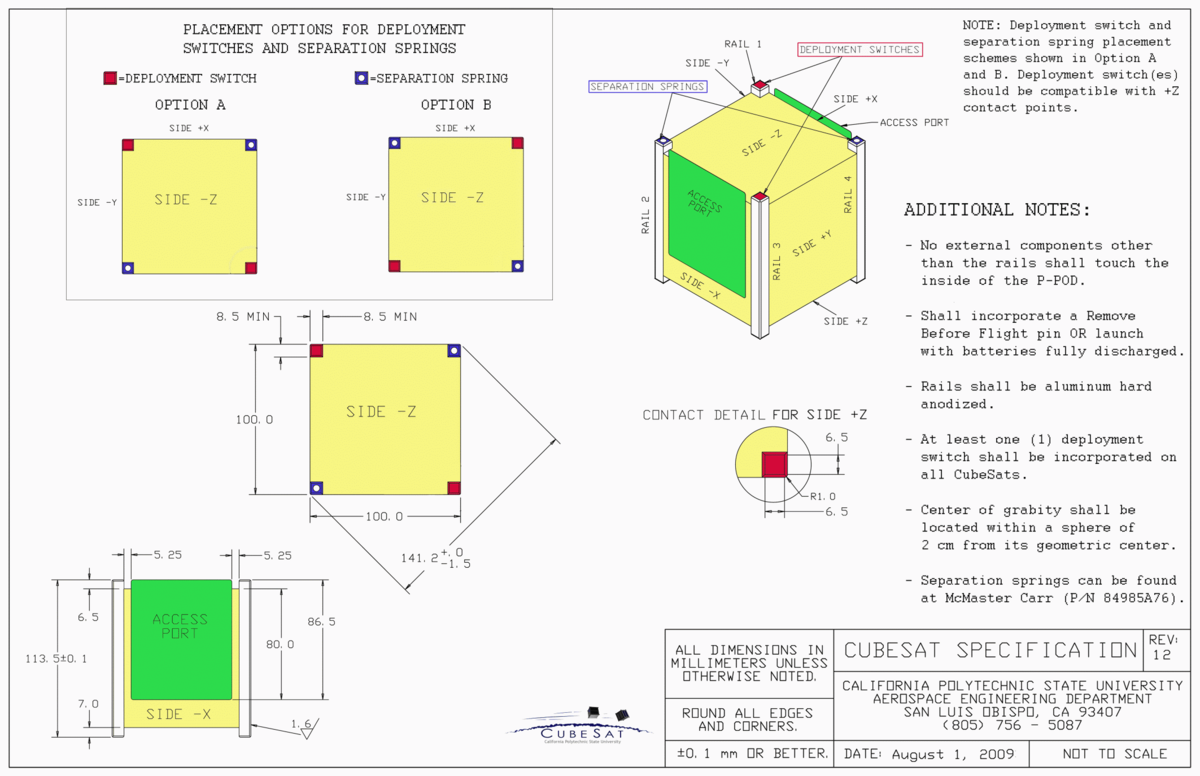
\includegraphics[width=1.0\linewidth]{cubesat_design.png}
	\caption{Спецификация спутника типа CubeSat}
	\label{fig:cubesat_design}
\end{sidewaysfigure}

Представленная на рисунке~\ref{fig:cubesat_design} техническая спецификация демонстрирует конструктивные особенности стандартного блока CubeSat формата 1U, разработанного в соответствии с требованиями California Polytechnic State University. Базовая конфигурация представляет собой кубический модуль размерами \(100 \times 100 \times 100\) мм с максимальной массой 1.33 кг.

Ключевыми конструктивными элементами являются алюминиевые направляющие рельсы шириной 8.5 мм, выполненные из сплавов 6061 или 7075 с обязательным твердым анодированием поверхности для предотвращения холодной сварки. Контактная поверхность торцевых направляющих составляет не менее \(6.5 \times 6.5\) мм для обеспечения механического взаимодействия с соседними блоками в развертывающем устройстве.

Система развертывания включает deployment switches (переключатели развертывания) и separation springs (разделительные пружины), расположенные на противоположных гранях модуля. Переключатели развертывания обеспечивают блокировку активации бортовых систем на глубину до 0.75 мм с рабочим ходом не более 2.0 мм и усилием до 3 N. Разделительные пружины типа McMaster Carr P/N 84985A76 создают усилие от 0.5 до 1.5 lbf с минимальным ходом 0.05 дюйма, обеспечивая безопасное разделение блоков после развертывания.

Техническая документация предписывает размещение центра масс в пределах сферы радиусом 2 см от геометрического центра блока. Внешние компоненты на боковых гранях не должны выступать более чем на 6.5 мм от плоскости направляющих рельсов. Система контактных деталей для стороны +Z включает access port и специализированные крепежные элементы с резьбой M5×0.8.

Представленная спецификация соответствует стандарту CubeSat Design Specification Rev. 14.1 и обеспечивает совместимость с развертывающими устройствами типа P-POD, E-SSOD и ISIPOD. Модульная архитектура позволяет объединение нескольких 1U блоков в конфигурации 2U, 3U, 6U и 12U для реализации более сложных космических миссий.
